\documentclass{report}
\usepackage[T1]{fontenc} % Fontes T1
\usepackage[utf8]{inputenc} % Input UTF8
\usepackage[backend=biber, style=ieee]{biblatex} % para usar bibliografia
\usepackage{csquotes}
\usepackage[portuguese]{babel} %Usar língua portuguesa
\usepackage{blindtext} % Gerar texto automaticamente
\usepackage[printonlyused]{acronym}
\usepackage{hyperref} % para autoref
\usepackage{graphicx}
\usepackage{amsmath} % matemática
\usepackage{amssymb} % matemática
\usepackage{float}

\addbibresource{bibliografia.bib}

\begin{document}
%%
% Definições
%
\def\titulo{Trabalho de Aprofundamento 2, Grupo 3}
\def\data{20 de Abril de 2018}
\def\autores{Rodrigo Rosmaninho, Eurico Dias}
\def\autorescontactos{(88802) r.rosmaninho@ua.pt, (72783) dias.eurico@ua.pt}
\def\versao{1}
\def\departamento{DETI}
\def\empresa{Universidade de Aveiro}
\def\logotipo{ua.pdf}
%
%%%%%% CAPA %%%%%%
%
\begin{titlepage}

\begin{center}
%
\vspace*{50mm}
%
{\Huge \titulo}\\ 
%
\vspace{10mm}
%
{\Large \empresa}\\
%
\vspace{10mm}
%
{\LARGE \autores}\\ 
%
\vspace{30mm}
%
\begin{figure}[h]
\center
\includegraphics{\logotipo}
\end{figure}
%
\vspace{30mm}
\end{center}
%
\begin{flushright}
\versao
\end{flushright}
\end{titlepage}

%%  Página de Título %%
\title{%
{\Huge\textbf{\titulo}}\\
{\Large \departamento\\ \empresa}
}
%
\author{%
    \autores \\
    \autorescontactos
}
%
\date{\data}
%
\maketitle

\pagenumbering{roman}

%%%%%% Agradecimentos %%%%%%
% Segundo glisc deveria aparecer após conclusão...
\renewcommand{\abstractname}{Agradecimentos}
\begin{abstract}
Gostaríamos de agradecer a: 

\begin{description}
	\item[Professor Auxiliar António José Ribeiro Neves], pelas excelentes aulas sobre Python e Sockets, e esclarecimento de dúvidas.
	
	\item[Professor Auxiliar João Paulo Barraca], regente da U.C., pelo esclarecimento de variadas dúvidas sobre este trabalho de aprofundamento, ajuda com problemas com a conexão à sonda, e extensão do prazo de entrega.
	
	\item[Professor Auxiliar António Manuel Adrego da Rocha ], pela aula elucidante que nos foi dada sobre \LaTeX no semestre passado, sem a qual não conseguiríamos ter completado este relatório.
\end{description}
\end{abstract}


\tableofcontents
\listoffigures


%%%%%%%%%%%%%%%%%%%%%%%%%%%%%%%
\clearpage
\pagenumbering{arabic}

%%%%%%%%%%%%%%%%%%%%%%%%%%%%%%%%%
%%%%%%%%%%%%%%%%%%%%%%%%%%%%%%%%%

\chapter{Introdução}
\label{chap.introducao}

Este trabalho, desenvolvido no âmbito da \ac{uc} de Laboratórios de Informática, constou na criação de um cliente em Python com a capacidade de aceder remotamente a uma sonda de temperatura, humidade, e vento instalada pelos docentes. 

O cliente recebe dados em \ac{json} a cada 10 segundos e regista-os num ficheiro em formato \ac{csv} (\textbf{data.csv}), imprimindo, eventualmente, alguns avisos no terminal conforme as condições climatéricas.\newline

Para além disso, as mensagens entre o cliente e o servidor são encriptadas usando \ac{aes}-128 com uma chave de encriptação calculada por ambos os intervenientes através do algoritmo de Diffie-Hellman. No entanto, as mensagens estão sujeitas a sofrer corrupção foi, por isso, necessário acrescentar alguma robustez ao código.\newline

\hfill

Para simplificar a resolução do trabalho, o grupo decidiu dividir o código-fonte em 4 ficheiros Python (excluíndo os ficheiros utilizados para a elaboração de testes unitários), cada um com a sua função e vários métodos. 

Outra decisão do grupo foi a inclusão de cores nas impressões para o terminal, de forma a salientar erros e informações importantes.\newline 

O projeto do code.ua associado a este trabalho pode ser consultado em \url{http://code.ua.pt/projects/labi2018-ap2-g3}

%%%%%%%%%%%%%%%%%%%%%%%%%%%%%%%%%
%%%%%%%%%%%%%%%%%%%%%%%%%%%%%%%%%

\chapter{Metodologia}
\label{chap.metodologia}
Apresentação e descrição da metodologia utilizada para a realização do projeto e obtenção de resultados.

%%%%%%%%%%%%%%%%%%%%%%%%%%%%%%%%%

\section{main.py}

\subsection{Objetivos}
O ficheiro \textbf{main.py} consiste na lógica principal de comunicação com o servidor, receção e interpretação do \ac{json}, e escrita de valores num ficheiro em formato \ac{csv}.

Ou seja, o ficheiro tem as funções:
\begin{itemize}
	\item Conectar ao servidor por sockets \ac{tcp} usando funções de \textbf{net.py}.
	\item Establecer comunicação encriptada de acordo com o guião (CONNECT/READ) para trocar os parametros necessários para a criptografia por \ac{dh}. (usar funções de \textbf{security.py}.
	\item Validar e ler respostas do servidor em \ac{json}.
	\item Determinar se é necessário avisar o utilizador das condições climatéricas.
	\item Escrita dos dados gerados em formato \ac{csv} para o ficheiro \textbf{data.csv}.
\end{itemize}

\subsection{Métodos}

\subsubsection{Método main()}
Este método contem a lógica principal de todo o projeto.
É este que é chamado quando se executa o ficheiro \textbf{main.py}.
Pode ser dividido em duas partes:
\begin{itemize}
	\item Establecimento de conexão (encriptada) com o servidor.
	\item Receção e utilização contínua dos dados recebidos.
\end{itemize}

Sendo assim, a lógica do método segue a seguinte ordem:
\begin{enumerate}
 \item Establecer um socket \ac{tcp} com o porto \textbf{8080} de \textbf{xcoa.av.it.pt}
  \item Chamar a função \textbf{DHInitialValues()} do \textbf{security.py} para obter os parametros A, p, g enviar "CONNECT <A, p, g>" ao servidor.
  \item Receber o parametro B do servidor e apartir dele gerar a chave de encriptação usando \textbf{DHGetSecret()} do \textbf{security.py}. Também é recebido um token.
  \item Enviar a primeira mensagem encriptada com \ac{aes} ao servidor ("READ <token>"), para que o servidor começe a enviar valores provenientes da sonda. 
\end{enumerate}

\hfill


É ainda necessecário tomar em consideração o facto das transmissões poderem sofrer corrupção e, por isso, não ser possível desencriptar e interpretá-las.

A vasta maioria das mensagens recebidas durante o tempo de vida do programa são atualizações dos valores provenientes da sonda e podem, se ocorrer corrupção, ser ignoradas.\newline

As mensagens recebidas durante a troca de parametros criptográficos são, no entanto, cruciais, visto que se, por exemplo, ocurrer corrupção na mensagem que contém os valores \textbf{token} e \textbf{B}, o cliente não conseguirá calcular a chave de encriptação usada pelo servidor e não será possivel desencriptar as mensagens que forem recebidas posteriormente. \newline

Desta forma, as partes do código referentes a operações de desencriptação de mensagens foram 'envoltas' em blocos \textbf{try/except}, já que a corrupção torna a desencriptação impossível dada a discrepâncias no número de bits.

Como já foi dito, todas as exceções originadas em processos de desencriptação de mensagens não cruciais levam a que a mensagem seja ignorada.

Em contrapartida, erros em mensagens cruciais levam à execução do método \textbf{handleFatalError()}, que imprime um erro e reinicia o programa.


\subsubsection{Método handleFatalError()}
Este método é chamado pelo \textbf{main()} quando ocorre corrupção numa mensagem enviada pelo servidor que é crucial ao funcionamento do resto do programa.

Como tal, imprime uma mensagem de 'erro fatal' e chama o método \textbf{main()} para que o programa seja 'reiniciado'.

\subsubsection{Método getInfo()}
O presente método é chamado pelo \textbf{main()} para que se averigue as possíveis condições climatéricas existentes no momento de execução do programa, baseado nos valores obtidos pela sonda e enviados pelo servidor, e recomenda vestuário e/ou ações de acordo. A função imprime uma linha por cada tipo de valor (temperatura, humidade e vento).
\newline
Como as condições meteorológicas podem variar drasticamente apenas em períodos de tempo significativametne maiores que 10 segundos (intervalo entre as mensagens), não é necessário imprimir avisos num intervalo de tempo tão curto. Para além disso, os valores que chegam são imediatamente impressos no terminal em forma de tabela, o que tornava o \textit{output} do programa bastante confuso. Com isto, a função informa acerca das condições climatéricas aquando da primeira mensagem que chega do servidor, e só volta a avisar passados 5 minutos.

\subsubsection{Método initialExchange()}
Este método é chamado pelo \textbf{main()} quando é necessário efetuar a troca inicial de parâmetros criptográficos com o servidor, ou seja, enviar \textbf{CONNECT A,p,g} e receber os valores \textbf{token} e \textbf{B}. 
Estes são devolvidos pelo método, para que no \textbf{main()} estes possam ser usados para calcular a chave de encriptação a usar.

\subsubsection{Métodos restantes}
\begin{itemize}
  \item \textbf{isValidJSON()} -> retorna \textbf{True} se o argumento constituir \ac{json} válido.
  \item \textbf{readJSON()} -> retorna um dicionário equivalente a um objeto \ac{json} dado como argumento.
  \item \textbf{hasError()} -> retorna \textbf{True} se o argumento (mensagem enviada pelo servidor em \ac{json}) constituir uma mensagem de erro.
\end{itemize}

%%%%%%%%%%%%%%%%%%%%%%%%%%%%%%%%%

\section{net.py}

\subsection{Objetivos}
O ficheiro \textbf{net.py} consiste num conjunto de métodos essenciais para a conexão e troca de mensagens com o servidor remoto.

\subsection{Métodos}
\subsubsection{Método tcpConnect()}
Este método establece a conexão por \ac{tcp} ao servidor cujo endereço e porto aceita como argumentos, returnando o socket recém-criado.

Para além disso também guarda o socket como variável global para que as restantes funções de \textbf{net.py} possam fazer uso dele sem terem de o aceitar como argumento.

Se não for possível establecer a conexão, o programa imprime um erro (que pede ao utilizador que verifique o estado da sua ligação à internet) e sai.

\subsubsection{Método tcpSend()}
Este método codifica os dados a ser enviados (fornecidos por argumento) em base64 ou \ac{utf8} caso os dados estejam encriptados ou não, respetivamente.\newline
De seguida, os dados recém-codificados são enviados para o servidor.

\subsubsection{Método tcpRead()}
Este método recebe uma nova mensagem do servidor e retorna-a.

%%%%%%%%%%%%%%%%%%%%%%%%%%%%%%%%%

\section{security.py}
\subsection{Contexto}

%%%%%%%%%%%%%%%%%%%%%%%%%%%%%%%%%%%%%%%%%%%%%%%%%%%%%%%%%%%%%%%%%

\subsubsection{Troca do segredo partilhado}
A geração e troca de chaves partilhadas com o algoritmo de Diffie-Hellmann é um método que possibilita a troca de segredos a partir de duas ou mais entidades desconhecidas uma da outra, por via de um canal de comunicação inseguro.\newline
Em resumo, este método pressupõe a utilização de propriedades e fórmulas matemáticas bem conhecidas, que garantem tanto a consistência do resultado entre ambas as partes negociadoras, assim como a dificultação da aplicação de engenharia reversa ao processo de geração dos valores resultantes da aplicação destas fórmulas.

\subsubsection{Encriptação}
Após ser gerado o segredo, é possível agora a \textbf{cifra das mensagens}, para que assegure um nível relativamente satisfatório de segurança (dada a importância dos dados que são transmitidos neste trabalho) na troca de informação entre o cliente e o servidor. Como algoritmo de cifra, foi nos dado como requisito a utilização do \textbf{\ac{aes}}, com chaves de comprimento 16 (em bytes).

%%%%%%%%%%%%%%%%%%%%%%%%%%%%%%%%%%%%%%%%%%%%%%%%%%%%%%%%%%%%%%%%%

\subsection{Objetivos}
O ficheiro \textbf{security.py} , tal como o nome indica, contém os métodos necessários para garantir algum nível de segurança entre as mensagens \ac{json} trocadas. Resumidamente, os métodos principais neste ficheiro permitem:

\begin{itemize}
\item Gerar valores recorrendo ao algoritmo de Diffie-Hellmann para a negociação da chave a utilizar na cifra da informação
\item Computar uma chave dos primeiros 16 carateres hexadecimais a partir dos valores \ac{dh} calculados pelo servidor, recorrendo a uma síntese \ac{md5}
\item Encriptar mensagens \ac{aes} recorrendo ao algoritmo de cifras contínuas \ac{aes}-128 com a chave gerada anteriormente
\item Com a mesma chave, decifrar a informação que chega do servidor.
\end{itemize}
Os métodos secundários, que completam os métodos principais, possibilitam:

\begin{itemize}
\item Descobrir valores que complementam a geração dos parâmetros de Diffie-Hellmann
\item Retirar o excipiente de uma mensagem \ac{json} previamente decifrada
\item Verificar a primalidade e paridade de um número
\end{itemize}
Adicionalmente, este ficheiro pode ser executado por si só para a conexão manual ao servidor. O código no final do ficheiro permite depurar alguns tipos de problemas menos óbvios.

\subsection{Métodos}
\subsubsection{Método DHGetInitialValues()}
Este método gera os parâmetros iniciais para a primeira conexão ao servidor. O fluxo desta função é a seguinte:

\begin{itemize}
\item Gera os parâmetros para o cálculo de $A$: computa um número primo aleatório $p$ e encontra uma base geradora de campo deste primo respetiva $g$
\item Calcula um inteiro aleatório privado $a$
\item Calcula $A=g^a\pmod{n}$
\item Retorna um tuplo da forma $(A,p,g)$
\end{itemize}

Antes da inicialização do processo, é necessária a geração dos parâmetros por meio de funções de pseudo-aleatoriedade e do cálculo de valores intermédios. A geração destes parâmetros, tanto do número primo $p$, como do gerador de campo $g$, foi realizada a partir de uma adaptação do standard \ac{rfc} (Request for Comments) 2631, do \ac{ietf}\cite{rfc}/\ac{ansi} X9.42\cite{ansi}. O parâmetro $q$ é um fator primo de $p$ e é originado realizado operações aritméticas com diferentes valores a partir de sínteses \ac{sha}-256 de uma string de bits pseudo-aleatória (chamada de \textit{seed}), seguindo de operações bit a bit. O parâmentro $p$ é gerado a partir de q e também é gerado de forma semelhante, garantindo que $p$ é um primo com fator $q$.
\newline
De notar que a adaptação do standard considerou os requisitos descritos no enunciado e as restrições do servidor, que limita o tamanho do número primo (de 32 a 128 bits) do mínimo de 512 bits descritos neste \ac{rfc}/\ac{ansi}, para que os algoritmos recomendados no standard produzam um resultado satisfatório. Adicionalmente, com o módulo de criptografia para Python3 mais recente (pycryptodome), os métodos da função de síntese para a geração dos parâmetros recomendada (já obsoleta) não é disponibilizada. Com isto, as seguintes alterações aos algoritmos de geração foram realizadas:
\begin{itemize}
    \item Encurtamento do tamanho da String (denominada seed) para 100 bits;
    \item Alteração das funções de síntese sobre valores intermédios de \ac{sha}-1, de 160 bits, para \ac{sha}256, de 256 bits;
    \item Alterações a valores incluídos que dependem do ponto anterior (para que as operações bit a bit produzam resultados válidos).
\end{itemize}
Depois da geração destes valores, é gerado um valor $g$, que é um gerador do subgrupo (do campo de Galois de $p$) multiplicativo de ordem $q$, que satisfaz a equação $g^j\pmod{p}\neq1$, sendo $j$ um número inteiro tal que $j=\frac{p-1}{q}$.
\newline
De seguida gera-se um número inteiro pesudo-aleatório $a$, no intervalo $[2^{q-1},q-2]$ e calcula-se o parâmetro final $A$ tal que $A=g^a\pmod{n}$, que é retornado pela função juntamente com $p$ e $g$ na forma de um tuplo $(A,p,g)$.

\subsubsection{Método \_checkPrime(num, seg=50)}

Como consequência dos algoritmos estandardizados pelo \ac{rfc}/\ac{ansi}, muitos dos números computados são primos (o parâmetro $p$, por exemplo). Considerando que a maior parte deles possuem um tamanho relativamente considerável ($p$, neste trabalho, tem 127 bits), é necessário um algoritmo que não despendesse grande parte do tempo de geração, e ainda assim, no entanto, satisfatoriamente robusto, para a verificação de primalidade dos números e parâmetros.\newline
Com isto, utilizou-se o \textbf{método de primalidade de Miller-Rabin}\cite{miller}, explicitado no standard. Este \textbf{método probabilístico} permite a verificação da pseudo-primalidade de um inteiro com base no \textbf{pequeno teorema de Fermat}\cite{fermat} e, consequentemente, no \textbf{teorema de Euler-Fermat}\cite{euler}. Semelhante a todos os métodos probabilísticos, tem sempre uma margem de erro para falsos positivos. Este erro, segundo o standard, não deverá ser menor que $\frac{1}{4^{\text{seg}}}$. O parâmetro de segurança, \textit{seg}, consiste no nível de passagens sobre a prova do número, garantindo menor erro.\newline
Resumidamente, este método faz uma aplicação do método probabilístico acima sobre um inteiro(num) e retorna um valor booleano para discernir a provável primalidade de um número.

\subsubsection{Método DHGetSecret(\textit{p}, \textit{B})}
Este método, resumidamente, computa o segredo partilhado tal que $\textit{key}=B^{a}\pmod{p}$, sendo $p$ o número primo gerado anteriormente e $B$ um valor gerado pelo servidor, de maneira análoga à do método \textbf{DHGetInitialValues()}.\newline
De seguida, retorna uma síntese hexadecimal MD5 do valor obtido (32 carateres, pois a síntese \ac{md5} retorna 16 bytes, na qual cada byte são 2 nibbles), para posterior utilização em cifras assimétricas.

\subsubsection{Método encrypt(chave, msg)}
O presente método recebe uma chave e uma mensagem, e aplica o algoritmo de cifras assimétricas \ac{aes}-128, sendo que a chave tem que possuir exatamente 16 bytes. Como a chave recebida do método \textbf{DHGetSecret()} retorna uma representação hexadecimal de 128 bits, como já foi explicado, a chave irá ter, tecnicamente, 32 bytes (em string de carateres). Portanto, como foi requerido pelo enunciado deste trabalho, é necessário forçar o tamanho de 16 bytes selecionando apenas os primeiros 16 da chave dada.\newline
Depois, é feita a encriptação da mensagem em blocos de 16 bytes (o tamanho dos blocos é definido pela chave). O último bloco da mensagem pode não ter o tamanho correto. Para que este fique com o tamanho correto, é necessário adicionar um excipiente. Neste trabalho, foram adicionados espaços em branco.\newline
Esta mensagem, quando totalmente encriptada, está pronta para ser codificada em base64 por outra função e, seguidamente, enviada para o servidor.

\subsubsection{Método decrypt(chave, msg)}
Este método recebe uma chave e uma mensagem \ac{json} encriptada, e decifra o conteúdo com o mesmo algoritmo de cifra utilizado para a encriptação. Adicionalmente, é necessário retirar-lhe o excipiente para que fique exatamente igual à mensagem de encriptação. O excipiente foi retirado tendo em conta que as mensagens enviadas pelo servidor, quando encriptadas, são sempre mensagens em \ac{json}. Portanto, a forma mais simplificada de obter a mensagem inicial consiste em percorrer a mensagem do fim para o início e contar os carateres até que se identifique o carater "\}". Depois, é só retornar o subconjunto da mensagem até à diferença do tamanho da mensagem com o número de carateres contados.\newline
Finalmente, é retornada a mensagem desencriptada, para posterior processamento pelo resto do programa.

%%%%%%%%%%%%%%%%%%%%%%%%%%%%%%%%%

\chapter{Testes}
\label{chap.testes}

\section{main.py}
Para este ficheiro foram feitos testes unitários para os métodos:
\begin{itemize}
  \item \textbf{isValidJSON()}
  \item \textbf{readJSON()}
  \item \textbf{hasError()}
\end{itemize}

\hfill

Para o fazer, primeiro foram declaradas diversas variáveis com strings \ac{json} válidas e inválidas (para passar como argumento a \textbf{isValidJSON()}), e, para cada string \ac{json} válida, um dicionário correspondente (para comparar com o resultado de \textbf{readJSON()} com a string \ac{json} usada como argumento).\newline

Por último, foram criadas variáveis correspondentes a strings \ac{json} válidas com e sem o formato de uma típica mensagem de erro enviada pelo servidor (para passar como argumento a \textbf{hasError()}).\newline

Não foram feitos testes unitários para as restantes funções visto que essas dependiam de comunicação com o servidor.

\section{security.py}

Os testes unitários foram realizados para a totalidade das funções, exceto a função \textbf{\_checkParity}, por ser bastante simples.\newline
Tentou-se que os testes fossem individualizados para cada função, sem qualquer chamada ou utilização de valores entre elas. No entanto, da forma como foram implementadas, estas agem como complementares umas da outras, e, por esta razão, muitos dos testes utilizam valores e chamadas de outras funções criadas neste mesmo ficheiro.\newline
Os testes para este ficheiro foram escritos noutro ficheiro, denominado \textbf{test\_security.py}.\newline
Passando à explicitação dos testes:
\begin{itemize}
\item No que toca ao método \textbf{DHGetInitialValues()}, o parâmetro $A$ não pode ser negativo, sendo que apenas estamos a lidar com números inteiros positivos. O parâemtro p não pode ser negativo nem menor que dois. Finalmente, o g tem que estar congruente com os algoritmos utilizando, sendo que $g\pmod{p} < 2\land g\pmod{p}\neq p-1$.
\item Em relação ao método \textbf{DHGetSecret()}, foi averiguado se a chave não era nula e se possui exatamente 32 bytes hexadecimais (como string), ou seja, 16 bytes. Adicionalmente, foi emulado o cálculo (simplificado) dos parâmetros Diffie-Hellmann por parte do servidor servidor, para que se conseguisse testar a igualdade entre as chaves obtidas das "duas" partes.
\item Para o método \textbf{\_checkPrime()}, foi testada a robustez do algoritmo aplicado: testou-se a primalidade de um número negativo, do 0, do 1 e do 2, assim como um número primo óbvio, um número não primo óbvio, entre outros.
\item Os testes para o método \textbf{\_unpadJSON()} foram simples: testou-se a mensagem vazia, a string com apenas o carater "\}" (retorna a string vazia, como é suposto), um \ac{json} vazio com excipiente numérico e um \ac{json} com uma entrada, também este com um excipiente numérico.
\item No que toca às funções \textbf{encrypt()} e \textbf{decrypt()}, estas foram combinadas numa única "função de testes": tentou-se encriptar e desencriptar logo de seguida um json de uma entrada de teste, e também uma string vazia.
\end{itemize}
Posto isto, a execução deste \textit{set} de testes unitários é bem sucedida, não encontrando qualquer erro.
%%%%%%%%%%%%%%%%%%%%%%%%%%%%%%%%%
%%%%%%%%%%%%%%%%%%%%%%%%%%%%%%%%%

\chapter{Conclusões}
\label{chap.conclusao}
\section{Resultados}
No que toca aos resultados obtidos pela execução do programa, este funciona corretamente.\newline
Como mostra a \autoref{img.resultterm}, observa-se que os dados que são enviados pelo servidor são corretamente impressos no terminal, juntamente com o aviso inicial das condições climatéricas de momento. Face à corrupção das mensagens enviadas pelo servidor, o programa avisa dessa mesma corrupção, ignora o seu conteúdo e continua a ser executado, como pretendido.

\begin{figure}[H]
\centering
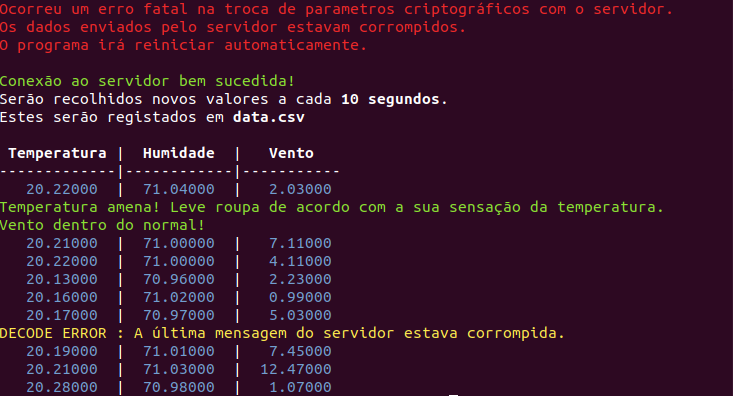
\includegraphics[scale=0.5]{resultterm.png}
\caption{\textit{Output} do programa no terminal.}
\label{img.resultterm}
\end{figure}

Na figura \autoref{img.resultcsv}, pode-se verificar que o ficheiro \ac{csv} foi preenchido com a informação das mensagens que foram enviadas pelo servidor, com a adição de um campo com a data aquando do seu registo (ou o \textit{timestamp}), que só faz sentido neste caso, pois os dados meteorológicos apenas têm relevância quando são registados temporalmente.

\begin{figure}[H]
\centering
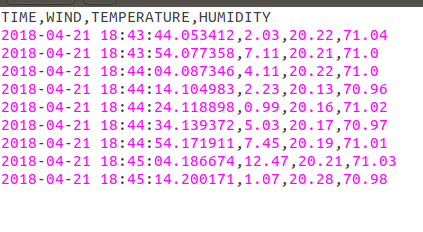
\includegraphics[scale=0.8]{resultcsv.png}
\caption{Resultado dos dados presistidos num ficheiro \ac{csv}.}
\label{img.resultcsv}
\end{figure}

Acerca dos testes unitários, foi executado o \textbf{pytest} tanto nos testes do ficheiro \textbf{test\_main.py} como nos do \textbf{test\_security.py}. Respetivamente, como podemos observar nas figuras \autoref{img.unitmain} e \autoref{img.unitsecurity}, não foi encontrado qualquer problema na execução destes.

\begin{figure}[H]
\centering
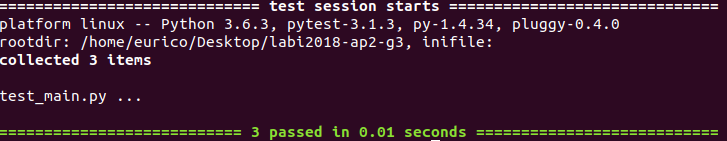
\includegraphics[scale=0.45]{unitmain.png}
\caption{Resultado dos testes unitários sobre o ficheiro \textbf{main.py}.}
\label{img.unitmain}
\end{figure}

\begin{figure}[H]
\centering
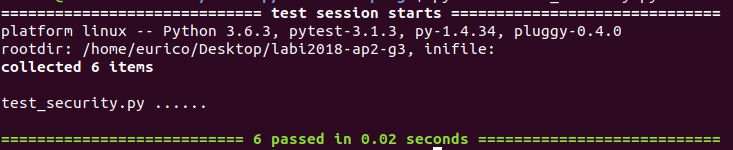
\includegraphics[scale=0.45]{unitsecurity.png}
\caption{Resultado dos testes unitários sobre o ficheiro \textbf{security.py}.}
\label{img.unitsecurity}
\end{figure}

\section{Conclusão}
Este trabalho de aprofundamento permitiu aos autores do mesmo consolidar a implementação de sockets, manipulação de estruturas de ficheiros ou mensagens \ac{json} e \ac{csv}, e também a aplicação de cifras simétricas por blocos recorrendo a \ac{aes}, na linguagem de programação Python. Para além disso, forneceu uma ideia geral na negociação de um segredo partilhado pelo método de Diffie-Hellmann, e também na implementação de testes unitários a métodos/funções não triviais, que dependem de outras na sua execução.

\chapter*{Contribuições dos autores}
A contribuição individual para o trabalho foi a seguinte:

\textbf{Rodrigo Rosmaninho}
\begin{itemize}
\item main.py (exceto método getInfo() e persistência dos dados em ficheiro \ac{csv})
\item net.py
\item colors.py
\item test\_main.py (Testes unitários)
\item Relatório: Estrutura inicial, agradecimentos, introdução, partes respetivas do trabalho
\end{itemize}

\textbf{Eurico Dias}
\begin{itemize}
\item main.py - getInfo() e persistência de dados em ficheiro \ac{csv}
\item security.py
\item test\_security.py (Testes unitários)
\item Relatório: Partes respetivas do trabalho, conclusões, acrónimos e bibliografia
\end{itemize}
Segue-se a percentagem da contribuição total:
\begin{itemize}
\item \textbf{Rodrigo Rosmaninho} - 50\%
\item \textbf{Eurico Dias} - 50\%
\end{itemize}

%%%%%%%%%%%%%%%%%%%%%%%%%%%%%%%%%
\chapter*{Acrónimos}
\begin{acronym}
\acro{aes}[AES]{Advanced Encryption Standard}
\acro{ansi}[ANSI]{American National Standards Institute}
\acro{csv}[CSV]{Comma-Separated Values}
\acro{dh}[DH]{Diffie-Hellmann}
\acro{ietf}[IETF]{Internet Engineering Task Force}
\acro{json}[JSON]{JavaScript Object Notation}
\acro{rfc}[RFC]{Request For Comment}
\acro{sha}[SHA]{Secure Hash Algorithm}
\acro{tcp}[TCP]{Transmission Control Protocol}
\acro{uc}[UC]{Unidade Curricular}
\acro{utf8}[UTF-8]{8-bit Unicode Transformation Format}
\end{acronym}


%%%%%%%%%%%%%%%%%%%%%%%%%%%%%%%%%
\printbibliography

\end{document}
